\chapter{État de l'Art de la Détection d'Anomalies pour la Maintenance Prédictive}
\label{chap:etat_art}
\thispagestyle{plain}

\section{Introduction}

Dans le contexte de l'Industrie 4.0, la maintenance prédictive (PdM) est devenue un impératif stratégique, visant à améliorer la fiabilité des équipements tout en maîtrisant les coûts opérationnels \cite{hector2024,achouch2022}. La PdM transcende la maintenance conditionnelle (CBM) par l'exploitation d'algorithmes sophistiqués d'analyse de données pour anticiper les défaillances \cite{ran2019}. La surveillance des vibrations est reconnue comme la modalité la plus performante pour l'évaluation de l'état des machines tournantes, permettant de capter les signatures précoces de défauts mécaniques \cite{tiboni2022,hassan2024}. Cependant, le déploiement de solutions d'intelligence artificielle (IA) traditionnelles reste entravé par leur complexité, leur coût et leur dépendance à des infrastructures cloud gourmandes en bande passante \cite{njor2024}. L'émergence du paradigme TinyML (Tiny Machine Learning) offre une alternative prometteuse, permettant l'exécution de modèles d'IA optimisés directement sur des microcontrôleurs (MCU) à ressources contraintes \cite{tsoukas2024}. Ce chapitre présente un état de l'art structuré des stratégies de maintenance, des techniques d'analyse vibratoire, des méthodes d'apprentissage automatique pour la détection d'anomalies, et du potentiel du TinyML pour les systèmes embarqués de PdM.

\section{Évolution de la maintenance industrielle}

L'évolution des stratégies de maintenance industrielle reflète une progression constante de l'approche réactive vers l'anticipative et l'optimisation, répondant à la complexité croissante des systèmes et à la nécessité de garantir la continuité de la production \cite{ran2019}. La normalisation, notamment par la norme européenne EN 13306 \cite{en13306}, fournit le cadre terminologique distinguant clairement les différents types d'actions.

\subsection{Typologie selon normes EN 13306 et ISO disponibles}

La \textbf{maintenance corrective} (ou réactive, \textit{Reactive Maintenance}, RM) est l'approche la plus ancienne, exécutée uniquement après qu'une défaillance se soit produite \cite{en13306,ran2019}. Bien qu'elle soit simple à planifier pour les actifs non critiques, elle conduit inévitablement à des temps d'arrêt non planifiés, à des coûts de réparation élevés (souvent trois fois plus importants que la maintenance planifiée) et à des risques de dommages collatéraux \cite{ran2019}.

La \textbf{maintenance préventive} (Preventive Maintenance, PM) vise à éviter la panne par des interventions planifiées, soit systématiquement (basées sur le temps ou l'usage), soit conditionnellement \cite{en13306,ran2019}. La maintenance préventive systématique réduit les aléas mais engendre un risque de sur-entretien coûteux et inutile, remplaçant des composants dont la durée de vie utile n'est pas encore atteinte \cite{ran2019}.

La \textbf{maintenance conditionnelle} (Condition-Based Maintenance, CBM) fonde ses décisions sur la surveillance d'indicateurs de l'état de l'équipement (\textit{condition monitoring}) \cite{en13306,iso17359}. La norme ISO 17359 fournit des lignes directrices détaillées pour l'établissement d'un programme de surveillance d'état, incluant la définition des objectifs, le choix des variables à mesurer, la détermination de la fréquence d'acquisition et l'établissement des critères d'alarme \cite{iso17359,achouch2022}. La CBM permet une intervention ciblée lorsque des signes de détérioration sont observés \cite{lee2014}.

La \textbf{maintenance prédictive} (Predictive Maintenance, PdM) est souvent perçue comme la forme la plus évoluée de la CBM \cite{achouch2022,lee2014,jardine2006}. Elle utilise des modèles d'analyse avancée (statistique, apprentissage automatique) pour non seulement diagnostiquer l'état actuel (diagnostic de panne) mais surtout pour effectuer le pronostic, c'est-à-dire l'estimation de l'évolution future de la dégradation et la prédiction de la durée de vie restante (Remaining Useful Life, RUL) \cite{lee2014,ran2019}.

Le concept de \textbf{Prognostics and Health Management (PHM)} est un cadre d'ingénierie qui intègre le diagnostic et le pronostic pour fournir une vue intégrée de l'état de santé de la machine, en vue de prendre des décisions de gestion de maintenance et de logistique optimales \cite{lee2014,achouch2022}. Le PHM est une fondation pour les concepts plus avancés comme les systèmes auto-maintenus (\textit{self-maintenance}) \cite{lee2014}.

\begin{figure}[ht]
\centering
\includegraphics[width=0.85\textwidth]{images/maintenance-types.png}
\caption{Évolution des stratégies de maintenance industrielle selon EN~13306:2017 \cite{en13306}}
\label{fig:maintenance_evolution}
\end{figure}

La figure~\ref{fig:maintenance_evolution} illustre la progression chronologique des approches de maintenance, de la plus réactive (maintenance corrective) vers la plus anticipative (PHM), reflétant l'intégration croissante de l'intelligence artificielle dans la gestion des actifs industriels.

\subsection{Coûts d'arrêt et enjeux PHM}

Les arrêts non planifiés constituent un enjeu économique majeur pour l'industrie. Les coûts horaires d'immobilisation peuvent varier considérablement selon le secteur, allant d'un minimum de 36\,000\,\$ par heure dans les biens de grande consommation (FMCG) jusqu'à 2,3\,millions de dollars par heure dans le secteur automobile, ou même 150\,000\,\$ par heure pour les petites et moyennes entreprises (PME) particulièrement vulnérables aux pertes de contrats \cite{siemens2024}. À l'échelle des 500 plus grandes entreprises mondiales, le coût total annuel des temps d'arrêt non planifiés est estimé à environ 1,4 trillion de dollars, soit 11\,\% de leurs revenus \cite{siemens2024}.

Face à ces enjeux, la PdM est devenue indispensable. Siemens estime que l'adoption complète des pratiques de PdM dans ces grandes organisations pourrait générer 388 milliards de dollars d'économies par une augmentation de 5\,\% de la productivité, et 233 milliards de dollars par une réduction de 40\,\% des coûts de maintenance \cite{siemens2024}.

\section{Analyse vibratoire des machines tournantes}

Pour les machines tournantes, la surveillance vibratoire est la méthode privilégiée pour l'évaluation de l'état des machines, permettant de capter les signatures précoces de défauts mécaniques \cite{iso20816-1,hassan2024,tiboni2022}. Les défauts mécaniques (balourd, désalignement, roulements endommagés) génèrent des signatures d'oscillations ou de mouvements qui sont capturées par des capteurs.

\subsection{Cadre normatif et évaluation (ISO 20816-1 et ISO 20816-3)}

L'évaluation et l'interprétation des données vibratoires sont structurées par les normes internationales de la série ISO 20816 \cite{iso20816-1}.

La norme \textbf{ISO 20816-1:2016} est le document fondamental qui établit les lignes directrices générales pour la mesure et l'évaluation des vibrations mécaniques des machines \cite{iso20816-1}. Elle s'applique aux mesures effectuées à la fois sur les parties tournantes (arbres) et non tournantes (paliers ou boîtiers) des machines complètes dans des conditions de fonctionnement stable, pour l'acceptation et la surveillance opérationnelle \cite{iso20816-1}. L'évaluation se fait généralement en considérant l'amplitude de la vibration large bande observée ainsi que les changements dans cette magnitude au fil du temps \cite{iso20816-1}. La norme fournit des conseils sur les quantités de mesure (déplacement, vitesse, accélération) et les techniques spécifiques pour la détection de problèmes dans les roulements \cite{iso20816-1}.

La norme \textbf{ISO 20816-3:2022} est un document sectoriel qui spécifie les exigences pour l'évaluation des vibrations des machines industrielles accouplées avec une puissance nominale supérieure à 15\,kW et des vitesses de fonctionnement comprises entre 120\,tr/min et 30\,000\,tr/min \cite{iso20816-3}. Elle fournit des critères d'évaluation pour les mesures effectuées \textit{in-situ} sur des paliers, des supports de palier, ou des carters \cite{iso20816-3}.

\textbf{Exigences de mesure :} La mesure des vibrations est réalisée par des transducteurs. Pour la surveillance, l'équipement doit être capable de mesurer la valeur efficace (\textit{root-mean-square}, r.m.s.) de la vibration large bande \cite{iso20816-3}. La plage de réponse en fréquence requise est d'au moins 10\,Hz à 1\,000\,Hz. Pour les machines dont la vitesse de rotation est faible (inférieure ou égale à 600\,tr/min), la limite inférieure de la plage de réponse plate ne doit pas dépasser 2\,Hz \cite{iso20816-3}.

\subsection{Capteurs et traitement du signal}

L'acquisition de données vibratoires est généralement effectuée par des accéléromètres \cite{hassan2024}. La tendance actuelle des dispositifs IoT et TinyML favorise l'utilisation d'accéléromètres basés sur la technologie MEMS (Micro-Electro-Mechanical Systems) \cite{hassan2024,arciniegas2025}. Ces capteurs sont appréciés pour leur faible coût, leur petite taille et leur faible consommation, les rendant idéaux pour l'intégration dans des dispositifs embarqués contraints \cite{hassan2024}.

Le signal vibratoire capturé est transformé et analysé pour en extraire des informations pertinentes \cite{hassan2024}. L'analyse est typiquement réalisée en plusieurs étapes \cite{tiboni2022}:
\begin{enumerate}
\item \textbf{Mesure et Pré-traitement} : Nettoyage des données pour gérer le bruit et les artefacts \cite{bagri2024}.
\item \textbf{Traitement du Signal} : Conversion du domaine temporel au domaine fréquentiel.
\item \textbf{Extraction de Caractéristiques} : Calcul d'indicateurs (statistiques, fréquentiels).
\item \textbf{Diagnostic/Pronostic} : Utilisation de modèles ML/DL pour l'identification ou la prédiction des défauts.
\end{enumerate}

\textbf{Analyse Fréquentielle (FFT) :} La transformation de Fourier rapide (FFT) est la technique la plus fondamentale et la plus utilisée, convertissant le signal temporel en spectre de fréquences \cite{cooley1965,hassan2024}. Elle permet d'identifier les fréquences caractéristiques des défauts (par exemple, le balourd à $1\times$ la fréquence de rotation, ou les fréquences spécifiques des défauts de roulements - BPFO, BPFI, etc.) \cite{matania2024,tiboni2022}. Ce principe est crucial car l'information sur l'état de santé est concentrée dans un nombre fini de fréquences prédictibles basées sur les spécifications du composant \cite{matania2024}.

\textbf{Analyse dans les domaines Temps-Fréquence :} Pour les signaux transitoires ou non-stationnaires (fréquents dans les machines tournantes à vitesse variable ou lors de défauts naissants), des méthodes plus avancées que la FFT sont nécessaires, telles que l'analyse par ondelettes (Wavelet Analysis) ou des méthodes basées sur l'analyse de l'enveloppe \cite{hassan2024}. Récemment, les méthodes de décomposition à échelle temporelle, comme l'Empirical Mode Decomposition (EMD) ou ses variantes, sont devenues essentielles car elles permettent de décomposer le signal en plusieurs composantes, facilitant l'extraction des informations complexes masquées dans les signaux bruts \cite{bagri2024}.

\section{Détection d'anomalies par apprentissage automatique}

La détection d'anomalies par apprentissage automatique (ML) est le moteur de la PdM, car elle permet d'identifier les schémas de comportement anormaux de manière autonome \cite{achouch2022,chandola2009}. L'efficacité des algorithmes dépend largement du type de données (étiquetées ou non) et des contraintes d'exécution.

\subsection{Apprentissage non supervisé}

Les méthodes non supervisées sont cruciales pour la PdM, car les données d'anomalies ou de défaillances sont souvent rares en milieu industriel \cite{arciniegas2025}. Ces algorithmes se concentrent sur la modélisation du comportement normal (\textit{normality performance}) et sur la détection de tout écart significatif.

\textbf{K-means :} Algorithme de clustering partitionnel simple et efficace \cite{macqueen1967}. Le K-means présente une complexité algorithmique réduite ($O(n \cdot k \cdot i \cdot d)$) et une faible empreinte mémoire, le rendant particulièrement adapté aux environnements à ressources contraintes. Pour la détection d'anomalies, un point est jugé anormal s'il est éloigné de son centroïde de cluster, ou si le cluster lui-même est de très petite taille \cite{arciniegas2025,chandola2009}. Des implémentations récentes ont démontré des latences inférieures à 20\,ms sur microcontrôleurs 32-bit pour la détection d'anomalies simples.

\textbf{Isolation Forest (IF) :} Cette technique non supervisée excelle dans l'isolation des points aberrants. Elle fonctionne en construisant des arbres de partitionnement aléatoire et se base sur l'idée que les anomalies, étant moins nombreuses et moins denses, sont séparées plus rapidement des données normales \cite{antonini2023}. Antonini \textit{et al.} \cite{antonini2023} ont implémenté un système IF sur un dispositif embarqué, démontrant sa capacité à réaliser une détection d'anomalie rapide (latence $<16$\,ms) dans des conditions industrielles extrêmes (-40°C à +85°C), soulignant sa pertinence dans l'écosystème TinyML.

\textbf{Autoencoders (AE) :} Les AE sont des réseaux neuronaux conçus pour apprendre une représentation compressée des données (encodage) et les reconstruire (décodage) \cite{ran2019}. Entraînés uniquement sur des données de fonctionnement normal, ils échouent à reconstruire les données d'anomalie avec précision, ce qui se traduit par une erreur de reconstruction élevée utilisée comme indicateur d'anomalie.

\subsection{Apprentissage supervisé}

Les méthodes supervisées sont utilisées pour le diagnostic et la classification lorsqu'un jeu de données de défaillance suffisant est disponible. Les cinq algorithmes les plus fréquemment employés pour la détection de défauts dans l'analyse de signaux vibratoires sont les Machines à Vecteurs de Support (SVM), les Réseaux Neuronaux Convolutifs (CNN), les réseaux Long Short-Term Memory (LSTM), les k-plus proches voisins (k-NN), et les Forêts Aléatoires (Random Forests, RF) \cite{bagri2024}.

\textbf{Machine à Vecteurs de Support (SVM) :} Les SVM sont des classifieurs binaires ou multiclasses cherchant à trouver l'hyperplan qui maximise la marge entre les classes \cite{jemmali2021,ran2019}. Leur efficacité a été démontrée pour le diagnostic des défauts mécaniques de machines tournantes, avec des précisions typiques de 90-95\% sur des datasets industriels.

\textbf{Réseaux Neuronaux Convolutifs (CNN) :} Les CNN, initialement conçus pour les tâches de vision, sont hautement performants pour l'extraction automatique de caractéristiques à partir de signaux bruts 1D ou de représentations 2D (spectrogrammes, images vibratoires) \cite{bagri2024}. Ils sont la base de nombreuses solutions d'apprentissage profond pour la PdM, y compris dans les architectures TinyML (par exemple, les CNN quantifiés à 8 bits pour la surveillance des machines-outils) \cite{langer2025}. Les CNN permettent d'atteindre des niveaux de précision très élevés (96-99\%) dans les tâches de classification de défauts \cite{langer2025}.

\textbf{Réseaux Long Short-Term Memory (LSTM) :} Le LSTM, une variante des réseaux neuronaux récurrents (RNN), excelle dans le traitement des données séquentielles et des séries temporelles, capturant efficacement les dépendances temporelles de la dégradation des équipements \cite{ran2019,bagri2024}. Cependant, les modèles LSTM sont souvent plus exigeants en mémoire que les CNN \cite{gupta2025}.

\subsection{Analyse comparative des approches}

\begin{table}[ht]
\centering
\caption{Comparaison des algorithmes ML pour la détection d'anomalies vibratoires. Les performances sont indicatives et varient selon le contexte d'application et l'implémentation.}
\label{tab:ml_comparison}
\small
\begin{tabular}{lcccc}
\toprule
\textbf{Algorithme} & \textbf{Complexité} & \textbf{Mémoire} & \textbf{Précision} & \textbf{Temps réel} \\
\midrule
K-means & $O(nkid)$ & Faible & Élevée & <20\,ms \\
Isolation Forest & $O(n\log n)$ & Moyenne & Très élevée & <16\,ms\cite{antonini2023} \\
SVM & $O(n^2)$ & Élevée & Très élevée & <50\,ms \\
CNN & $O(n \cdot m \cdot k)$ & Très élevée & Maximale & <100\,ms\cite{langer2025} \\
LSTM & $O(n \cdot h^2)$ & Très élevée & Très élevée & <150\,ms \\
Autoencoders & $O(n \cdot l \cdot h)$ & Élevée & Élevée & <80\,ms \\
\bottomrule
\end{tabular}
\end{table}

Le tableau~\ref{tab:ml_comparison} présente une comparaison objective des différents algorithmes selon les critères critiques pour l'implémentation embarquée. Les algorithmes non supervisés (K-means, Isolation Forest) offrent un compromis intéressant entre performance et ressources, particulièrement adapté aux contraintes des microcontrôleurs.

\section{Paradigme TinyML et intelligence embarquée}

Le TinyML représente un changement de paradigme fondamental dans le déploiement de l'IA en environnement industriel, étendant l'Edge Computing jusqu'aux microcontrôleurs à ultra-faible consommation \cite{tsoukas2024,njor2024}. Ce concept permet d'exécuter des modèles d'apprentissage automatique directement sur le dispositif de détection, au plus près de la source de données.

\subsection{Définition et architecture}

Le TinyML est une technologie émergente permettant l'exécution d'algorithmes complexes d'apprentissage automatique sur des dispositifs matériels fortement contraints, tels que les microcontrôleurs 32 bits \cite{tsoukas2024}. Ces dispositifs sont caractérisés par une mémoire très limitée (typiquement moins de 256\,KB de SRAM disponible pour l'inférence) et une capacité de traitement réduite, imposant l'optimisation extrême des modèles \cite{njor2024}.

L'architecture TinyML se distingue des systèmes PdM traditionnels basés sur le cloud, où les données sont d'abord collectées, puis transmises hors du site pour un traitement sur des serveurs haute performance \cite{njor2024}. En TinyML, le traitement se fait sur le dispositif même (\textit{on-device}), ce qui apporte des avantages cruciaux pour la PdM \cite{tsoukas2024}.

\textbf{Avantages du TinyML pour la PdM :}
\begin{enumerate}
\item \textbf{Réduction de la Latence et Surveillance en Temps Réel :} Le traitement local élimine les délais de transmission au cloud, permettant une détection d'anomalies en temps quasi réel, essentielle pour réagir aux défauts naissants \cite{arciniegas2025,tsoukas2024}. Des études récentes ont atteint des latences de détection très faibles, telles que 15,4\,ms pour un modèle CNN sur un cœur Cortex M4F \cite{langer2025}.

\item \textbf{Efficacité Énergétique :} La minimisation de la communication sans fil avec le cloud, qui est une opération gourmande en énergie, réduit la consommation globale, permettant une autonomie prolongée pour les dispositifs alimentés par batterie \cite{tsoukas2024}.

\item \textbf{Confidentialité et Sécurité :} Les données sensibles restent sur le dispositif local, réduisant les risques liés à la transmission et au stockage centralisé, ce qui est impératif dans de nombreux contextes industriels réglementés \cite{njor2024,tsoukas2024}.
\end{enumerate}

\subsection{Contraintes et optimisations}

Les microcontrôleurs 32 bits offrent typiquement une quantité de mémoire SRAM très limitée pour le stockage et l'exécution du modèle. Cette contrainte dicte le choix des algorithmes et les méthodes d'optimisation.

\textbf{Techniques d'optimisation :}
\begin{itemize}
\item \textbf{Quantification :} Réduction de la précision numérique des poids et des activations du modèle, passant souvent d'une représentation en virgule flottante 32 bits (float32) à des entiers 8 bits (int8) \cite{tsoukas2024,krishnamoorthi2018}. Cela diminue drastiquement la taille de la mémoire requise et accélère le calcul, au prix d'une légère dégradation de la précision qui doit être gérée \cite{arciniegas2025,langer2025}.

\item \textbf{Pruning :} Élimination des connexions de poids faibles ou redondantes dans les réseaux de neurones, réduisant la complexité du modèle sans impact significatif sur la performance \cite{han2015}.

\item \textbf{Knowledge Distillation :} Transfert des connaissances d'un modèle complexe (teacher) vers un modèle plus simple (student), permettant d'obtenir des performances similaires avec moins de ressources \cite{hinton2015}.
\end{itemize}

\begin{figure}[ht]
\centering
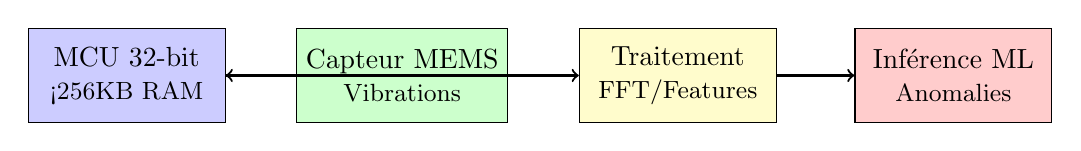
\begin{tikzpicture}[node distance=3.5cm, auto]
    % Nodes
    \node[draw, rectangle, fill=blue!20, minimum width=2.5cm, minimum height=1.2cm, align=center] (mcu) {MCU 32-bit\\{\small <256KB RAM}};
    \node[draw, rectangle, fill=green!20, minimum width=2.5cm, minimum height=1.2cm, right of=mcu, align=center] (sensor) {Capteur MEMS\\{\small Vibrations}};
    \node[draw, rectangle, fill=yellow!20, minimum width=2.5cm, minimum height=1.2cm, right of=sensor, align=center] (processing) {Traitement\\{\small FFT/Features}};
    \node[draw, rectangle, fill=red!20, minimum width=2.5cm, minimum height=1.2cm, right of=processing, align=center] (inference) {Inférence ML\\{\small Anomalies}};

    % Arrows
    \draw[->, thick] (sensor) -- (mcu);
    \draw[->, thick] (mcu) -- (processing);
    \draw[->, thick] (processing) -- (inference);
\end{tikzpicture}
\caption{Architecture générique TinyML pour la maintenance prédictive}
\label{fig:tinyml_architecture}
\end{figure}

\subsection{Implémentations récentes et état de l'art}

Les travaux TinyML pour la maintenance représentent une frontière active de recherche :

\begin{itemize}
\item \textbf{Antonini et al. (2023)} \cite{antonini2023} : Système Isolation Forest sur microcontrôleur pour environnements extrêmes (-40°C à +85°C), latence <16\,ms, démontrant la faisabilité du TinyML embarqué.

\item \textbf{Arciniegas et al. (2025)} \cite{arciniegas2025} : Dispositif IoT/TinyML pour vibrations moteurs, utilisant réseaux de neurones quantifiés (8-bit), précision 96.5\% avec latence minimale.

\item \textbf{Katib et al. (2025)} \cite{katib2025} : Deep learning embarqué pour IoT grand public, focus sur l'auto-apprentissage pour la détection d'anomalies en temps réel.

\item \textbf{Langer et al. (2025)} \cite{langer2025} : TinyML pour machines-outils CNC, approche hybride edge/cloud, démonstration sur cas industriel avec validation terrain.
\end{itemize}

Le cadre logiciel comme TensorFlow Lite Micro (TFLite Micro) est essentiel, agissant comme un outil de conversion de modèle et de moteur d'inférence pour permettre le déploiement sur les microcontrôleurs \cite{tflitemicro,tsoukas2024}. Le défi pour le TinyML en PdM demeure l'optimisation des flux de données vibratoires volumineux (nécessitant souvent FFT et extraction de caractéristiques à l'Edge avant l'inférence) pour maintenir la performance en temps réel sous les strictes contraintes matérielles \cite{gupta2025}.

\section{Analyse critique et positionnement}

\subsection{Analyse des solutions existantes}

La littérature récente sur la détection d'anomalies vibratoires embarquée révèle trois catégories d'approches :

\textbf{Solutions cloud-centrées :} Les architectures IIoT traditionnelles (capteur → gateway → cloud) dominent le marché industriel. Lee et al. \cite{lee2014} proposent des frameworks complets intégrant acquisition, transmission et analyse cloud. Ces solutions offrent des capacités analytiques étendues mais présentent des limitations : latence réseau (100\,ms-1\,s), dépendance connectivité, coûts récurrents (stockage/calcul), vulnérabilités cybersécurité.

\textbf{Approches edge computing :} L'edge computing rapproche le traitement de la source, avec des gains en latence (<50\,ms) et bande passante typiquement rapportés. Kong et al. \cite{kong2022} recensent des architectures edge pour l'industrie, utilisant des micro-serveurs pour l'analyse locale. Toutefois, ces plateformes restent coûteuses (>100€) et énergivores (5-10\,W) comparées aux MCU.

\textbf{Implémentations TinyML émergentes :} Les solutions TinyML démontrent la faisabilité technique avec des performances prometteuses (latences <20\,ms, précisions >90\%) mais restent limitées en termes de documentation d'implémentation et de validation terrain à grande échelle.

\subsection{Lacunes identifiées dans la littérature}

L'analyse critique révèle plusieurs manques :

\begin{enumerate}
\item \textbf{Accessibilité PME :} Les solutions restent complexes à déployer sans expertise IA/IoT. Aucune étude ne documente une implémentation "clé en main" pour techniciens maintenance.

\item \textbf{Validation terrain limitée :} La plupart des travaux utilisent des datasets publics (CWRU, IMS) plutôt que des validations industrielles réelles. Seuls Langer et al. \cite{langer2025} présentent des déploiements terrain documentés.

\item \textbf{Comparaisons incomplètes :} Absence de benchmarks standardisés TinyML/vibration. MLPerf Tiny \cite{banbury2021} ne couvre pas la maintenance prédictive.

\item \textbf{Documentation d'implémentation :} Les détails d'optimisation pour microcontrôleurs (quantification, gestion mémoire, organisation des données) restent souvent peu documentés dans la littérature académique.

\item \textbf{Coût total de possession :} Les études omettent l'analyse TCO incluant matériel, déploiement, maintenance et formation.
\end{enumerate}

\subsection{Synthèse et perspectives}

L'analyse de l'état de l'art révèle une opportunité significative pour le développement de solutions TinyML adaptées aux besoins et contraintes des PME. Les points clés identifiés sont :

\begin{enumerate}
\item \textbf{Maintenance prédictive :} Évolution nécessaire pour réduire les coûts d'arrêt (entre 36\,000\,\$ et plus de 2\,millions\,\$ par heure selon le secteur \cite{siemens2024}) mais inaccessible aux PME avec les solutions actuelles.

\item \textbf{Analyse vibratoire :} Modalité privilégiée pour les machines tournantes, normalisée (ISO 20816), riche en signatures de défauts et compatible avec des capteurs MEMS économiques.

\item \textbf{Algorithmes non supervisés :} Présentent un compromis intéressant entre simplicité computationnelle et efficacité de détection pour les microcontrôleurs contraints, particulièrement adaptés à l'absence de données de défauts étiquetées.

\item \textbf{Paradigme TinyML :} Permet l'IA embarquée sur microcontrôleurs 32-bit avec des contraintes sévères mais des performances suffisantes pour le temps réel industriel (<20\,ms).
\end{enumerate}

\subsection{Conclusion du chapitre}

L'analyse de l'état de l'art a mis en évidence le rôle critique de la maintenance prédictive, devenue un impératif économique pour l'industrie, en particulier pour contrer les coûts prohibitifs des arrêts non planifiés \cite{siemens2024}. La modalité d'analyse vibratoire, rigoureusement encadrée par la série de normes ISO 20816, s'impose comme la méthode la plus pertinente pour le diagnostic des machines tournantes \cite{iso20816-1,iso20816-3}. L'exploitation de ces données repose de plus en plus sur des modèles d'apprentissage automatique, avec un spectre allant des algorithmes sophistiqués d'apprentissage profond (CNN, LSTM) aux approches frugales non supervisées (K-means, Isolation Forest), le choix étant déterminé par la nature du problème et les contraintes d'implémentation \cite{bagri2024,antonini2023}.

Le paradigme TinyML offre la possibilité concrète de déporter l'intelligence artificielle directement sur des dispositifs de surveillance à microcontrôleur, permettant une détection d'anomalies en temps réel avec une faible latence, une haute efficacité énergétique et une confidentialité accrue \cite{tsoukas2024,njor2024}. Bien que la faisabilité technique ait été démontrée par des travaux récents \cite{arciniegas2025,antonini2023,langer2025}, une lacune persiste concernant la documentation détaillée des implémentations optimisées pour l'analyse vibratoire en temps réel sur architectures MCU contraintes, ainsi que leur accessibilité pour les PME \cite{oecd2021}.

Ces lacunes identifiées dans la littérature orientent vers le développement d'une solution TinyML adaptée aux contraintes des PME. Le chapitre suivant présentera la conception détaillée d'une architecture matérielle et logicielle répondant à ces défis.